\documentclass[11pt]{article}
\usepackage[margin=1in]{geometry}
\usepackage{amsmath,amssymb,amsthm}
\usepackage{graphicx}
\usepackage[T1]{fontenc}
\usepackage[colorlinks=true,linkcolor=blue,citecolor=blue,urlcolor=blue]{hyperref}

\newtheorem{theorem}{Theorem}
\newtheorem{corollary}{Corollary}

\title{\textbf{\large The Dual Membrane and Korselt Colour-Blindness\\
in Eisenstein Carmichael Ideals}}
\author{Ruqing Chen\\
\small GUT Geoservice Inc., Montreal, Quebec, Canada\\
\small \texttt{ruqing@hotmail.com}}
\date{June 2026}

\begin{document}
\maketitle

\begin{abstract}
\noindent
The preceding parts of this series mapped prime constellations and Carmichael pseudoprimes on the
$6N$ skeleton, the one-dimensional coordinate in which the primes $2$ and $3$ are stripped and every
surviving prime sits on a wing $6N\pm1$. This closing part lifts the construction to its
two-dimensional source, the Eisenstein integers $\mathbb{Z}[\omega]$ with their exact six-fold
symmetry, and asks what becomes of the Carmichael structure there. We prove a \emph{dual membrane
theorem}: no Eisenstein Carmichael number is divisible by the prime above $3$ (the ramified
$(1-\omega)$, norm $3$) or by the prime above $2$ (the inert $2$, norm $4$). The two exclusions are
independent and rest on different valuations---the first is a $3$-adic obstruction, the second a
$2$-adic parity obstruction---and together they show that the stripping of $2$ and $3$ that
\emph{defines} the $6N$ skeleton in one dimension is, in two dimensions, a \emph{theorem}: the
Carmichael structure expels the primes above $2$ and $3$ on its own. We then measure what survives
above the membrane. Classifying the admissible factors by their unit-invariant type (split, norm
$p\equiv1\bmod3$; versus inert, norm $q^2$, $q\equiv2\bmod3$, $q\ge5$) and enumerating Eisenstein
Carmichael ideals, we find the type-composition spectrum statistically indistinguishable from the null
model induced by the factor pool alone: the pure-split fraction is $0.663$ among Carmichael ideals
against $0.642$ under the norm constraint with the Korselt condition removed. Within the resolution
measured, the Korselt criterion is \emph{colour-blind}---it constrains only the multiplicative
congruence of norms and expresses no preference among factor types. The one-dimensional monochromatic
collapse has no type-level analogue in $\mathbb{Z}[\omega]$. We present this as a complete and honest
closure: a rigid exterior boundary, a structurally empty interior, and an explicit statement that this
is most plausibly the physical ceiling of the measurement programme.
\end{abstract}

\section{Introduction}
The $6N$ skeleton is the integers with the primes $2$ and $3$ removed. Every prime exceeding $3$ lies
on one of two wings, $6N-1$ or $6N+1$, of an integer centre $N$, and the thirty-six parts of
Volumes~I--III read the arithmetic of prime constellations, prime-rich sequences, and Carmichael
pseudoprimes through this single coordinate. The stripping of $2$ and $3$ was, throughout, a
\emph{definition}: we declared the centre and the wings by hand and measured what remained. The
construction earned its keep---it produced the membrane and parity laws of the Carmichael numbers
(Part~XXXVI)---but it always carried the question of why $2$ and $3$ should be the privileged
exceptions.

The answer, we believe, is geometric. The natural home of an exact six-fold symmetry is not the
integer line but the \textbf{Eisenstein integers} $\mathbb{Z}[\omega]$, $\omega=e^{2\pi i/3}$, the
triangular lattice whose unit group $\{\pm1,\pm\omega,\pm\omega^2\}$ is the six sixth-roots of unity.
An Eisenstein integer $a+b\omega$ has norm $N(a+b\omega)=a^2-ab+b^2$, and $\mathbb{Z}[\omega]$ is a
unique factorisation domain with genuine Eisenstein primes: rational primes $p\equiv1\pmod3$ split
into two conjugate primes of norm $p$; rational primes $q\equiv2\pmod3$ remain inert with norm $q^2$;
and $3$ ramifies as a unit times $(1-\omega)^2$, with $(1-\omega)$ of norm $3$. The two wings of the
$6N$ skeleton are, in this light, the shadow cast on a line by the six-fold lattice, and the
one-dimensional series may be read as a dimensional reduction of a two-dimensional object.

Carmichael numbers generalise here through the standard generalised Korselt criterion: a squarefree
ideal $I=\mathfrak{p}_1\cdots\mathfrak{p}_k$ is a Carmichael ideal when $N(\mathfrak{p}_i)-1\mid N(I)-1$
for every prime factor, the direct analogue of Korselt's rational criterion~\cite{Korselt} with primes
replaced by prime ideals. For a principal ideal $(\alpha)$ with $\alpha=\pi_1\cdots\pi_k$, this reads
$N(\pi_i)-1\mid N(\alpha)-1$, $N(\alpha)=\prod_iN(\pi_i)$. The objects are well defined; what is
essentially absent is any computational map of their macroscopic distribution.

This part draws that map and finds two facts of opposite character. The first is a rigid exterior
boundary: a \textbf{dual membrane theorem} stating that the ramified $(1-\omega)$ and the inert $2$
each divide no Eisenstein Carmichael number, one by a $3$-adic and the other by a $2$-adic obstruction.
Together they invert the logic of the series: the removal of $2$ and $3$, imposed by fiat in one
dimension, is forced in two. The $6N$ skeleton ceases to be an axiom and becomes a theorem. The second
fact concerns the interior, and is a negative result we regard as equal in value. The surviving factors
are of two unit-invariant types---split and higher inert---and one might expect, by analogy with the
violent monochromatic collapse of the one-dimensional left wing (Part~XXXVI), a comparable preference:
a two-dimensional collapse spectrum. There is none. Measured against the null model induced by the
factor pool alone, the Carmichael type composition shows no preference; above the membrane the
\textbf{Korselt criterion is colour-blind}.

We state the scope of the negative result plainly. Colour-blindness is asserted at the resolution
measured---the split-versus-inert type dichotomy and the coarse norm-residue labels of \S\ref{sec:cb}.
We do not claim a global symmetry beyond what was tested; we report that the natural type-level
collapse the one-dimensional theory would predict is absent.

A word on what is and is not new here, in keeping with the discipline of this series. Carmichael
ideals over rings of integers of number fields are a defined and studied object, generalised through
the Korselt-type condition $N(\mathfrak{p})-1\mid N(I)-1$~\cite{Steele2008,Bae2023}, and the exclusion
of the ramified and small inert primes---or facts from which it follows immediately---may well already
exist, in the abstract algebraic language of generalised Carmichael ideals, in this literature. We do
not claim the dual membrane as a new algebraic theorem. What this paper claims is the projection: the
recognition that the $6N$ skeleton's defining removal of $2$ and $3$ is, in the six-fold phase space
of $\mathbb{Z}[\omega]$, exactly the $2$-adic and $3$-adic geometric blockage of the primes above $2$
and $3$ from the Carmichael structure; and, above that boundary, the first large-scale empirical
mapping of the type-composition spectrum, which establishes the colour-blindness of the Korselt
criterion against an explicit null model. The membrane is, if one likes, an elementary corollary made
geometric; the colour-blindness measurement is, to our knowledge, drawn here for the first time.

Section~\ref{sec:inst} fixes conventions
and the instrument gate. Section~\ref{sec:mem} proves the dual membrane. Section~\ref{sec:cb} presents
the colour-blindness measurement and its null model. Section~\ref{sec:ledger} keeps the honest ledger,
and Section~\ref{sec:conc} closes the series.

\section{Conventions and the instrument}\label{sec:inst}
\paragraph{The lattice.}
We write $\alpha=a+b\omega$, $\omega=e^{2\pi i/3}$, $\omega^2=-1-\omega$, with norm
$N(a+b\omega)=a^2-ab+b^2=|a+b\omega|^2$, multiplicative. The unit group $\{\pm1,\pm\omega,\pm\omega^2\}$
is the six sixth-roots of unity at $0,60,\dots,300$ degrees; multiplication by a unit is a rotation by
a multiple of $60^\circ$. The primes are split (norm $p\equiv1\bmod3$), inert (norm $q^2$,
$q\equiv2\bmod3$), or ramified ($(1-\omega)$, norm $3$). We record the congruence on which
\S\ref{sec:mem} turns: \emph{the only Eisenstein prime norm not congruent to $1$ modulo $3$ is the
ramified $3$.} Split norms are $p\equiv1$; inert norms are $q^2\equiv1\pmod3$ for every $q\equiv2$
(and for $q=2$, norm $4\equiv1$); only the ramified $3\equiv0$ stands apart.

\paragraph{Eisenstein Carmichael ideals.}
A principal ideal $(\alpha)$, $\alpha=\pi_1\cdots\pi_k$ a product of $k\ge3$ distinct non-associate
Eisenstein primes, is an \emph{Eisenstein Carmichael ideal} when $N(\pi_i)-1\mid N(\alpha)-1$ for all
$i$, with $N(\alpha)=\prod_iN(\pi_i)$. Two features govern everything below. First, the criterion
depends on the factors \emph{only through their norms}: it is a statement about the multiset
$\{N(\pi_i)\}$, identical in form to the rational Korselt criterion on the multiset of Eisenstein prime
norms. Second, the Carmichael property is \emph{unit-invariant}: if $(\alpha)$ is Carmichael then so is
$(u\alpha)$ for any unit $u$. The Carmichael set is closed under the six-fold rotation.

\paragraph{The instrument and its gate.}
Because the programme rests on unbiased enumeration, we hold it to a gate: a quantity fixed by symmetry
must come out at its symmetric value exactly. Assign $\alpha$ the sextant
$\lfloor\arg(\alpha)/60^\circ\rfloor$. As the Eisenstein primes are closed under the six unit
rotations, their sextant occupancy must be exactly $\tfrac16$. An early sieve failed this gate,
returning occupancies near $0.158$ and $0.182$; the cause was diagnostic. A point of norm at most $X$
can have a coordinate as large as $|a|\approx1.155\sqrt X$ (the form $a^2-ab+b^2\le X$ is maximised in
$|a|$ near $b=a/2$), so a box of half-width $\sqrt X$ clips outer associates and breaks unit closure
asymmetrically. Enlarging the box to half-width $\lceil2\sqrt{X/3}\rceil$, and assigning the sextant by
exact integer rotation rather than floating-point argument, restores closure: the occupancy then reads
$0.16\overline{6}$ in every sextant with maximum deviation $0.000000$ at $X=4\times10^4,\,10^5,\,
2.5\times10^5$. We report the failure because it is the reason to trust what follows. Only after the
gate passes do we treat the enumerations as measurements.

\section{The dual membrane theorem}\label{sec:mem}
Throughout, $\alpha=\pi_1\cdots\pi_k$ is an Eisenstein Carmichael ideal, squarefree with $k\ge3$
distinct prime factors, satisfying $N(\pi_i)-1\mid N(\alpha)-1$ with $N(\alpha)=\prod_iN(\pi_i)$.

\begin{theorem}[ramified membrane, $3$-adic]\label{thm:ram}
The ramified prime $(1-\omega)$, of norm $3$, divides no Eisenstein Carmichael ideal.
\end{theorem}
\begin{proof}
Suppose $(1-\omega)\mid\alpha$. Then $3=N(1-\omega)$ is a factor norm, so $N(\alpha)\equiv0\pmod3$.
Since $k\ge3$, there is another prime factor $\pi$. Every non-ramified Eisenstein prime has norm
$\equiv1\pmod3$ (\S\ref{sec:inst}), so $N(\pi)\equiv1\pmod3$ and hence $3\mid N(\pi)-1$. Korselt
requires $N(\pi)-1\mid N(\alpha)-1$, so $3\mid N(\alpha)-1$, i.e. $N(\alpha)\equiv1\pmod3$,
contradicting $N(\alpha)\equiv0\pmod3$. Hence $(1-\omega)\nmid\alpha$.
\end{proof}

Every surviving factor, being non-ramified, carries a norm one above a multiple of $3$ and so forces
$N(\alpha)\equiv1\pmod3$ through the Korselt divisibility; the ramified prime, alone in carrying a norm
divisible by $3$, would force $N(\alpha)\equiv0\pmod3$, and the two cannot hold at once. This is the
exact two-dimensional lift of the one-dimensional barrier of Part~XXXVI, where $3\mid n-1$ governed
which wing a factor could occupy.

\begin{theorem}[inert-$2$ membrane, $2$-adic]\label{thm:inert}
The inert prime $2$, of norm $4$, divides no Eisenstein Carmichael ideal.
\end{theorem}
\begin{proof}
Suppose the inert $2$ divides $\alpha$, contributing the factor norm $4$. The remaining factor norms
are all odd: split norms $p\ge7$ are odd, inert norms $q^2$ ($q\ge5$) are odd, and the ramified $3$ is
odd (and excluded by Theorem~\ref{thm:ram}). Hence $N(\alpha)=4\cdot(\text{odd})\equiv0\pmod4$, so
$N(\alpha)-1$ is odd. Take any other factor $\pi$ (one exists, as $k\ge3$); its norm is odd, so
$N(\pi)-1$ is even. Korselt requires $N(\pi)-1\mid N(\alpha)-1$, an even number dividing an odd
number---impossible. Hence the inert $2$ does not divide $\alpha$.
\end{proof}

The obstruction here is a parity, independent of the residue modulo $3$. The inert $2$ is the unique
Eisenstein prime of even norm; its presence makes $N(\alpha)\equiv0\pmod4$, rendering $N(\alpha)-1$
odd, while every other factor contributes an even $N(\pi)-1$ that cannot divide it. Theorem~\ref{thm:ram}
turns on a congruence modulo $3$; Theorem~\ref{thm:inert} on a parity. The two membranes are logically
independent.

\begin{corollary}[dual membrane]\label{cor:dual}
Every Eisenstein Carmichael ideal is composed exclusively of split primes (norm $p\equiv1\pmod3$) and
higher inert primes (norm $q^2$, $q\equiv2\pmod3$, $q\ge5$). Equivalently $N(\alpha)\equiv1\pmod3$ and
$N(\alpha)$ is odd, for every Eisenstein Carmichael ideal.
\end{corollary}

The corollary is the precise sense in which the $6N$ skeleton becomes a theorem. In one dimension the
removal of $2$ and $3$ was a definition; in $\mathbb{Z}[\omega]$ the Carmichael structure removes the
primes above $2$ and $3$ by itself---the first by a $3$-adic congruence, the second by a $2$-adic
parity. No external coordinate is imposed; the skeleton is what the Korselt criterion leaves behind.

Direct enumeration confirms both theorems without exception. Among the $95$ Eisenstein Carmichael
ideals with $N(\alpha)\le10^7$ drawn from a factor pool of prime norms up to $250$---a pool that
explicitly \emph{includes} the ramified norm $3$ and the inert norm $4$---none has a factor of norm $3$
and none has a factor of norm $4$; every ideal satisfies $N(\alpha)\equiv1\pmod3$ and $N(\alpha)$ odd.
The full enumerated list, with each ideal's factor norms and split/inert type labels, is released as
the open dataset \texttt{eisenstein\_carmichael\_examples.csv} accompanying this paper (\S\ref{sec:conc}).
The smallest ideals, $N=637=7\cdot7\cdot13$, $\;1225=7\cdot7\cdot25$, $\;1729=7\cdot13\cdot19$,
illustrate the rule: every factor norm is $\equiv1\pmod3$ and odd, and the structure first appears, as
in the rational case, at three prime factors.

\section{Colour-blindness above the membrane}\label{sec:cb}
The dual membrane fixes the exterior. The interior question is whether, among the survivors, the
Korselt criterion prefers some combinations---whether there is a two-dimensional analogue of the
one-dimensional monochromatic collapse.

\paragraph{What a collapse would look like.}
Part~XXXVI found a violent one-dimensional asymmetry: numbers built entirely from one wing are crushed
relative to mixed ones. The two-dimensional counterpart uses the unit-invariant factor \emph{type} as
the colour. After the membrane each factor is split ($S$: norm $p\equiv1\bmod3$) or inert ($I$: norm
$q^2$, $q\equiv2\bmod3$, $q\ge5$), and an ideal has a type composition $(n_S,n_I)$. A collapse would
show as an over- or under-representation of the \emph{pure} states ($n_I=0$ or $n_S=0$) relative to
chance. The type is a genuine unit-invariant, read from the norm on which Korselt acts---not from the
geometric sextant, whose occupancy is forced to $\tfrac16$ by unit symmetry and so carries no
information about the criterion.

\paragraph{The null model.}
The bare counts cannot be read alone: the pool is unbalanced (below norm $250$, $50$ split ideals
against $26$ inert), and inert norms ($q^2\ge25$) are larger and exhausted sooner under a ceiling on
$N(\alpha)$. A pure-split--dominated population could merely reflect a split-rich pool. We isolate the
criterion's effect by a null model: from the same pool, draw $k$-subsets ($k=3,\dots,6$) subject only
to the norm ceiling $N(\alpha)\le2\times10^7$, with the Korselt condition \emph{removed}, and record
the type composition the pool and ceiling produce by themselves. The Carmichael population is the same
draw with Korselt imposed; any difference is the signature of the criterion.

\paragraph{The measurement.}
The two distributions are, to within the measured precision, the same:
\[
\begin{array}{lccc}
& \text{pure-split} & \text{mixed} & \text{pure-inert}\\[2pt]
\text{Eisenstein Carmichael} & 0.663 & 0.337 & 0.000\\
\text{Null (norm ceiling only)} & 0.642 & 0.354 & 0.004
\end{array}
\]
The pure-split fractions agree to about two percent, within the resolution of the measurement, and the
mixed fractions equally closely. The Korselt criterion moves the type composition essentially not at
all; the apparent dominance of pure-split states is an artifact of the split-rich pool, reproduced by
the null in which Korselt plays no role. Within this resolution, \textbf{the criterion is
colour-blind}: it constrains the multiplicative congruence of the norms and expresses no preference
among the surviving factor types. Figure~\ref{fig:main} displays both halves of the measurement: the
instrument gate on the left and the colour-blindness comparison on the right.

\begin{figure}[t]
\centering
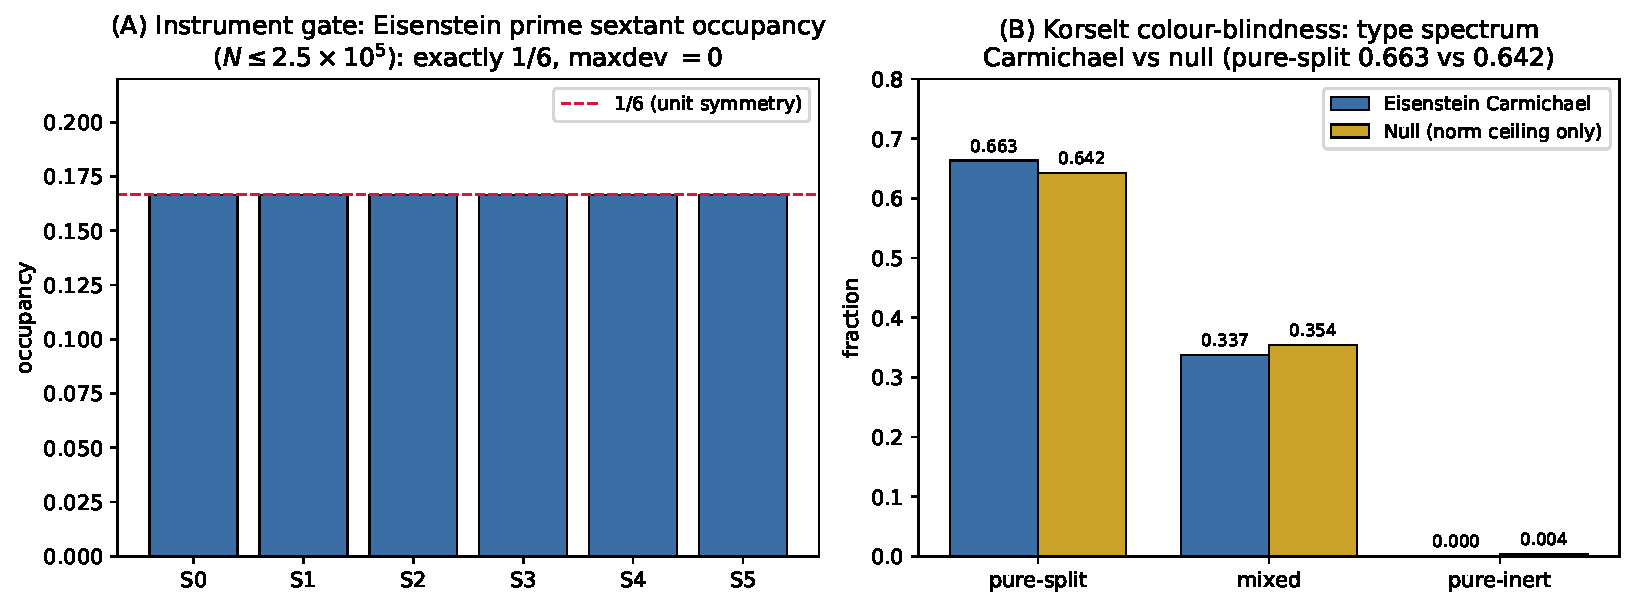
\includegraphics[width=\textwidth]{eisenstein_membrane_figures.pdf}
\caption{\textbf{(A)} Instrument gate: sextant occupancy of the Eisenstein primes with norm
$\le2.5\times10^5$, exactly $\tfrac16$ in every sextant (maximum deviation $0.000000$), confirming the
sieve respects the six-fold unit symmetry. \textbf{(B)} Korselt colour-blindness: the type-composition
spectrum of Eisenstein Carmichael ideals (split / mixed / inert) against the null model induced by the
factor pool and the norm ceiling alone, with the Korselt condition removed. The two agree to within the
measured precision (pure-split $0.663$ versus $0.642$); the criterion expresses no preference among the
surviving factor types.}
\label{fig:main}
\end{figure}

The near-vanishing of the pure-inert column in \emph{both} rows must not be mistaken for a third
membrane. It is not a structural exclusion but a consequence of the norm ceiling: inert norms are
squares $q^2\ge25$, three or more of which multiply past the ceiling before any Korselt question is
asked, and the null---which knows nothing of Korselt---produces the same near-zero. The honest-ledger
discipline of Part~XXXVII applies: an emptiness the null model also produces is sparsity, not law.

\paragraph{Scope.}
The colour-blindness is established at the resolution measured---the split-versus-inert dichotomy, the
natural unit-invariant colour suggested by the membrane. We have not examined every finer label and do
not assert a global symmetry of the Korselt criterion beyond what was tested. What we report is that
the one structure the one-dimensional theory would lead one to expect, a type-level monochromatic
collapse, is absent: measured against its own null model, the two-dimensional Carmichael population
shows no type preference.

\section{The honest ledger}\label{sec:ledger}
\paragraph{What is proved.} The dual membrane theorem is unconditional and elementary:
Theorem~\ref{thm:ram} rests on a single congruence, Theorem~\ref{thm:inert} on a single parity. We make
no claim that their difficulty is anything but slight; their interest is structural---the two primes
removed by hand in one dimension are removed by the Korselt criterion itself in two, each by its own
valuation.

\paragraph{What is measured.} The colour-blindness is a negative result reported against an explicit
null model, the pure-split fraction $0.663$ for Carmichael ideals against $0.642$ for the null. We
regard it as the genuine finding of the second half of the paper, of a piece with the series' practice
of treating a well-founded negative result as a result.

\paragraph{What is likely already known.} We are candid that neither theorem is likely to be new.
Carmichael ideals over rings of integers are a defined and studied object, generalised from the
rational theory of Carmichael numbers~\cite{AGP}: Carmichael numbers in number rings were treated by
Steele~\cite{Steele2008}, and the structure of Carmichael ideals and rings over Dedekind domains was
developed more recently by Bae, Hu, and Sha~\cite{Bae2023}. The exclusion of the ramified and small
inert primes from Eisenstein Carmichael ideals---or facts from which it follows---may well already be
contained, in the abstract algebraic language of those treatments, in this literature; we do not claim
the dual membrane as a new algebraic theorem. The contribution we claim is the one this series has
always claimed: not the mechanism but its placement---the identification of the dual membrane as the
exact two-dimensional source of the $6N$ skeleton's defining exclusion, rendered as concrete $2$-adic
and $3$-adic geometric blockages in the six-fold phase space, and the computational map of the
Carmichael population above it, including the colour-blindness measurement.

\paragraph{What was corrected along the way.} The colour-blindness was nearly mis-read twice, and both
near-misses are recorded. A raw count of pure-split against mixed first looked like a collapse; the null
model showed it was the factor pool. A vanishing pure-inert column first looked like a third membrane;
the null model showed it was the norm ceiling. The instrument itself failed its symmetry gate before it
passed (\S\ref{sec:inst}). We keep these so the result carries its corrections, not a cleaned-up account
of them.

\paragraph{What is not claimed.} No global symmetry of the Korselt criterion beyond the tested
resolution; no infinitude or counting statement about the Eisenstein Carmichael ideals; no novelty for
the membrane theorems themselves.

\section{Conclusion: the boundary and the free interior}\label{sec:conc}
The Eisenstein integers were proposed as the two-dimensional source of the $6N$ skeleton, and the
Carmichael structure bears the proposal out in a single clean figure: a rigid boundary around a free
interior. The boundary is the dual membrane---the prime above $3$ excluded by a $3$-adic congruence,
the prime above $2$ by a $2$-adic parity---so that the removal of $2$ and $3$, the founding gesture of
the series, imposed by definition in one dimension, is in two dimensions a theorem. The skeleton is not
a coordinate we chose; it is what the Korselt criterion leaves standing. The interior is free: above the
membrane, measured against its own null model, the criterion shows no preference among the surviving
factor types, and the monochromatic collapse that organised the one-dimensional theory has no
type-level analogue here.

We close the series on this result, and state plainly that it is most plausibly the ceiling of the
measurement programme. The $6N$ lens was built to read the density of primes and pseudoprimes on a
skeleton of residues, and its leverage was always specific to that structure. Lifted to its natural
home, the lens reproduces its own foundation as a theorem and then finds the space above that
foundation to be, at the resolution measurement can reach, without further structure of the kind the
lens was built to detect. That is a complete result rather than an exhausted one: an exterior law
proved, an interior emptiness measured and not papered over. Across thirty-eight parts the programme set
out to chart a single arithmetic mechanism to the edge of what measurement establishes, and to be
honest about that edge. Here the edge is reached in both directions at once---the boundary made rigid,
the interior shown free---and the atlas is complete.

\paragraph{Data and code availability.}
The reproducer \texttt{eisenstein\_dual\_membrane.py} (instrument gate, dual-membrane verification, and
colour-blindness null test, standard library only) and the dataset
\texttt{eisenstein\_carmichael\_examples.csv} (the enumerated Eisenstein Carmichael ideals with factor
norms and split/inert type labels) are openly available at
\url{https://github.com/Ruqing1963/6N-eisenstein-dual-membrane}. The
script regenerates the instrument gate ($1/6$ occupancy to machine precision), the dual-membrane
confirmation (zero ideals using the ramified norm $3$ or the inert norm $4$), and the colour-blindness
comparison ($0.663$ pure-split for the Carmichael population against $0.642$ under the null); any reader
can reproduce the null-deviation result directly from these files.

\begin{thebibliography}{9}
\bibitem{Korselt} A. Korselt, \emph{Probl\`eme chinois}, L'interm\'ediaire des math\'ematiciens
\textbf{6} (1899), 142--143.
\bibitem{AGP} W. R. Alford, A. Granville, and C. Pomerance, \emph{There are infinitely many Carmichael
numbers}, Ann. of Math. \textbf{139} (1994), 703--722.
\bibitem{Steele2008} G. A. Steele, \emph{Carmichael numbers in number rings}, J. Number Theory
\textbf{128} (2008), 910--917.
\bibitem{Bae2023} S. Bae, S. Hu, and M. Sha, \emph{On the Carmichael rings, Carmichael ideals and
Carmichael polynomials}, Colloq. Math. \textbf{171} (2023), 1--17.
\bibitem{P36} R. Chen, \emph{Topological Collapse and Asymmetric Divergence of Carmichael Pseudoprimes
on the $6N$ Skeleton} (Part XXXVI), Zenodo, 2026,
\href{https://doi.org/10.5281/zenodo.20611583}{doi:10.5281/zenodo.20611583}.
\end{thebibliography}

\end{document}
